%	Copyright (C) 2008, 2009 Julian M. Kunkel
%
%	This file is part of PIOsimHD.
%
%	PIOsimHD is free software: you can redistribute it and/or modify
%	it under the terms of the GNU General Public License as published by
%	the Free Software Foundation, either version 3 of the License, or
%	(at your option) any later version.
%
%	PIOsimHD is distributed in the hope that it will be useful,
%	but WITHOUT ANY WARRANTY; without even the implied warranty of
%	MERCHANTABILITY or FITNESS FOR A PARTICULAR PURPOSE.  See the
%	GNU General Public License for more details.
%
%	You should have received a copy of the GNU General Public License
%	along with PIOsimHD.  If not, see <http:%www.gnu.org/licenses/>.


\documentclass[
     11pt,         % font size
     a4paper,      % paper format
     BCOR10mm,     % binding correction
     DIV14,        % stripe size for margin calculation
     liststotoc,   % table listing in toc
     bibtotoc,     % bibliography in toc
     idxtotoc,     % index in toc
     parskip       % paragraph skip instad of paragraph indent
     ]{scrreprt}   %report
\usepackage{times}

\usepackage[numbers]{natbib}

\font\klingon=klinz

\citeindextrue

%%%%%%%
\usepackage[left=2.1cm,top=1.8cm,right=2.1cm,bottom=2.4cm]{geometry}
\usepackage{courier}

\usepackage[USenglish]{babel}
% Input encoding
\usepackage[utf8]{inputenc} 
% Font encoding
\usepackage[T1]{fontenc}
% Index-generation
%\usepackage{makeidx}
% Einbinden von URLs:
\usepackage{url}
% Special \LaTex symbols (e.g. \BibTeX):
\usepackage{doc}
% Include Graphic-files:
\usepackage{graphicx}
\usepackage{amsmath}
% Include doc++ generated tex-files:
%\usepackage{docxx}
% Include PDF links
\usepackage[pdftex, bookmarks=true]{hyperref}
\usepackage{enumitem}
\usepackage{fancybox}
\usepackage{rotating}
%%%%%%%%%%%%%%%%%%%%%%%%%%%%%%%%%%%%%%%%%%%%%%%%%%%%%%%%%%%%

% OTHER SETTINGS:
%\usepackage[pdftex,colorlinks,linkcolor=blue]{hyperref}
\newcommand{\myTitle}[0]{
Simulation of Parallel I/O and MPI Communication with a Discrete Event Simulator
}

\newcommand{\cmd}[1]{\texttt{#1()}}

\newcommand{\fatRot}[1]{
  \begin{turn}{-90}
   \textbf{#1}
  \end{turn}
 }

\usepackage{color}
\usepackage{listings} \lstset{numbers=left, numberstyle=\tiny, numbersep=5pt} \lstset{language=C} 
\lstset{frame=shadowbox, numbers=none,  rulesepcolor=\color{black}}

% Pagestyle:
\pagestyle{headings}

% Choose language
\newcommand{\setlang}[1]{\selectlanguage{#1}\nonfrenchspacing}

\newcommand{\includescalepngs}[1]{
\includegraphics[scale=0.5]{../bilder/#1}
}

\newcommand{\client}{ \begin{enumerate}[label=C\arabic{*}, ref=C(\arabic{*})]  }


\hypersetup{
	pdftitle = {\myTitle},
	pdfsubject = {Technical Report},
	pdfauthor = {Julian Martin Kunkel},
	pdfkeywords = {Parallel File Systems, High Performance Computing, MPI, Simulation}
}

\begin{document}
\begin{titlepage}

\vspace*{1cm}
\begin{center}
\textbf{
\Large Ruprecht-Karls-Universität Heidelberg\\
\smallskip
\Large Institut für Informatik\\
\smallskip
\Large Arbeitsgruppe Parallele und Verteilte Systeme\\
\smallskip
}

\vspace{3cm}

\textbf{\large Technical Report} 

\vspace{0.5\baselineskip}
{\huge
\myTitle
}
\end{center}

\vfill

{\large
\begin{tabular}[l]{ll}
Julian Martin Kunkel\\
January 2009
\end{tabular}
}

\end{titlepage}

\tableofcontents

\chapter{Introduction}
\section{Clusters}
* Cluster, Nodes, Bottleneck

\section{Message Passing Interface}
** Communication

\section{Parallel file systems}
** Optimizations, ROMIO


\section{Goals}
\begin{itemize}
\item Fast prototyping of new algorithms, for I/O optimization and MPI
\item Reveal bottlenecks.
\item Teaching, better understanding of observed system behavior
\item Test applications on different cluster hardware i.e. GRIDs
\item Simple but extendible models which can be selected on demand.
   Explicit abstraction from the real world complexity (for instance TCP Sliding Windows algorithm).
   However, similar results (runtime) to real world experiments should be possible
\item Usage of common tools to analyze simulation results.
\item Real OpenSource Software
\end{itemize}

\section{State of the Art}
\subsection{Simulators}
** Paraver / Dimemas
** Starfish
** The Network Simulator
** GTNets
** NCTUns 4.0

%* Performance optimization
%** ROMIO: Two-Phase-I/O, 

\subsection{Models}
Realistic Communication Model for Parallel Computing on Cluster.
http://i.cs.hku.hk/~clwang/papers/model-iwcc99.ps



\chapter{Model}

\begin{figure}%[!htbp]
  \centering
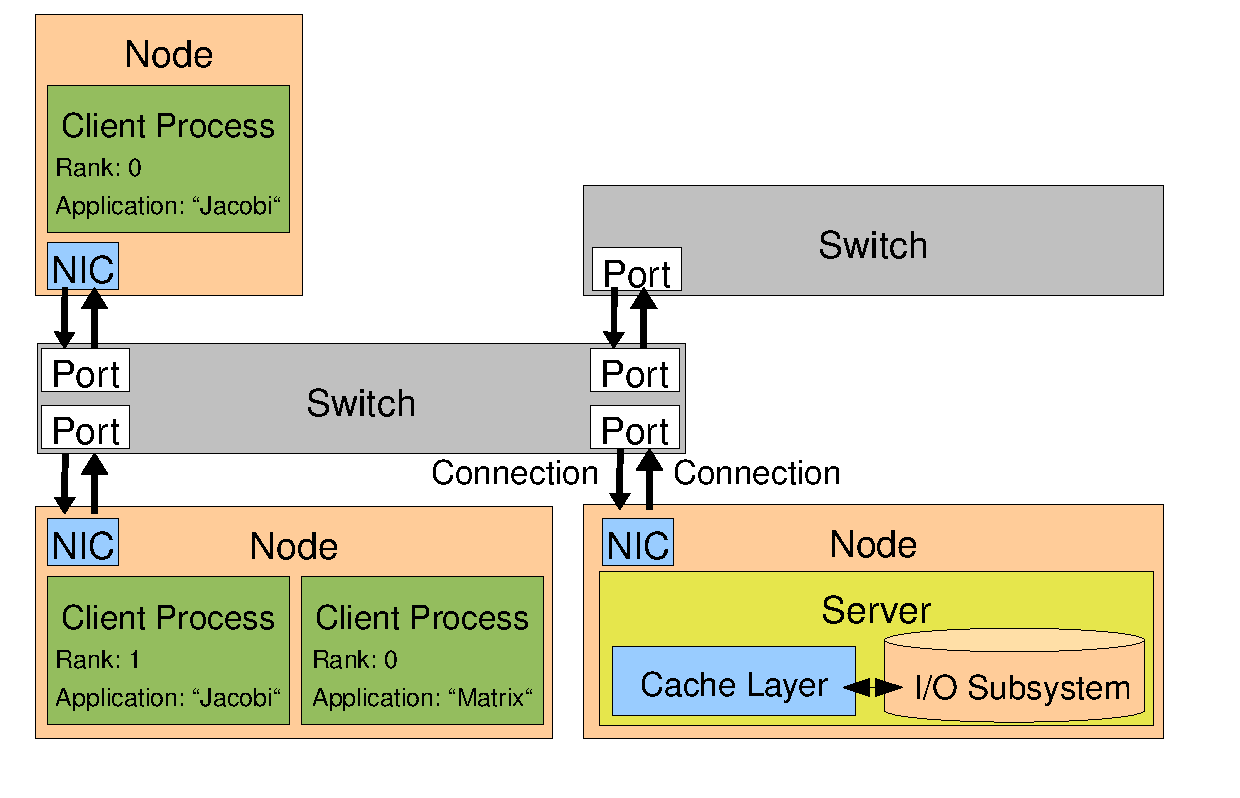
\includegraphics[scale=0.75]{Images/cluster-model.pdf}
    \caption{Example cluster component model}
    \label{fig:cluster-model}
\end{figure}

\begin{figure}
  \centering
\includegraphics[scale=0.75]{Images/cluster-relation.pdf}
    \caption{UML diagram showing the relations between cluster components}
    \label{fig:cluster-relation}
\end{figure}


* Exchangable component behavior
  Interfaces are not completely specified and can be modified as required.

\section{Elementary Components}
\subsection{Node}
\subsection{Network Interface Card (NIC)}
\subsection{Client Process}
\subsection{Server Process}
\subsection{Server Cache Layer}
\subsection{I/O Subsystem}
\subsection{Switch}
\subsection{Port}
\subsection{Connection}

\section{Application}
\subsection{Program}
\subsection{Command}

\section{Logical Files}



\chapter{PIOsimHD Package}
\section{Source Code}
* Split into Model, GUI, Simulation
\section{Provided Binaries/Scripts} %Example Usage
piosimhd
tau2slog2
jumpshot




\chapter{Design}

\section{Design Principles}
* Reflection
* Annotations
* Basic Model Classes contain Data
* Generation of Model, on run-time the simulator instanciates classes depending on the user configuration implementing such a model. The model is fixed during simulation.

\section{Model Generation}
* builder classes assist to build a (normal) model on the fly.

CommandToSimulationMapper.txt
\begin{verbatim}
# define the command groups and the contained implementations and the simulator implementations
# each row is either a set of commands which are implemented or the actual set of implementation classes for these commands.
+de.hd.pvs.piosim.model.program.commands.Compute
de.hd.pvs.piosim.simulator.component.Commands.Global.Dummy
de.hd.pvs.piosim.simulator.component.Commands.Compute.Time

#define a group:
+de.hd.pvs.piosim.model.program.commands.Send,de.hd.pvs.piosim.model.program.commands.Receive,de.hd.pvs.piosim.model.program.commands.Sendrecv # so it defines a group of commands at once which belong together.
de.hd.pvs.piosim.simulator.component.Commands.Global.Dummy,de.hd.pvs.piosim.simulator.component.Commands.Global.Dummy,de.hd.pvs.piosim.simulator.component.Commands.Global.Dummy
de.hd.pvs.piosim.simulator.component.Commands.SendReceive.Rendezvous.RendezvousSend,de.hd.pvs.piosim.simulator.component.Commands.SendReceive.Rendezvous.RendezvousRcv,de.hd.pvs.piosim.simulator.component.Commands.SendReceive.Rendezvous.RendezvousSendrecv

...
\end{verbatim}

ModelToSimulationMapper.txt
\begin{verbatim}
# This file describes the existing model component of a given type i.e. "Node" the available Model implementations and mapping to the simulation implementation.
+ClientProcess
de.hd.pvs.piosim.model.components.ClientProcess.ClientProcess = de.hd.pvs.piosim.simulator.component.ClientProcess.GClientProcess

+IOSubsystem
de.hd.pvs.piosim.model.components.IOSubsystem.SimpleFlash = de.hd.pvs.piosim.simulator.component.IOSubsystem.GSimpleFlash
de.hd.pvs.piosim.model.components.IOSubsystem.SimpleDisk = de.hd.pvs.piosim.simulator.component.IOSubsystem.GSimpleDisk
de.hd.pvs.piosim.model.components.IOSubsystem.RefinedDiskModel = de.hd.pvs.piosim.simulator.component.IOSubsystem.GRefinedDiskModel

...
\end{verbatim}


\section{XML Generation}
* serialization of annotated attributes

\section{Run a Simulation}
\subsection{Event processing}
* Future events are handled inside the simulator in a priority queue sorted on the time the activities start
* Event handling inside the components

\subsection{Debugging}
* start java with enabled assertions (\texttt{"`-ea"'} flag)
* the ConsoleLogger class or Component Logger class prints debugging output on the console
depending on the class (similar to \texttt{log4j}) and depending on the IDs of BasicComponents.
\begin{verbatim}
# The file is grouped in two sections:
ClassNamesToTrace
# The canonical class names which shall be debugged:
de.hd.pvs.piosim.simulator.component.ClientProcess.GClientProcess

ComponentIDsToTrace
# The component IDs which shall be debugged:
77
78
\end{verbatim}

\subsection{Simulation speed}
* 100.000 events/second
* Simulation Speed, remove assertions 15 seconds vs. 3.5 seconds (debug/assertions) and 1.8 seconds with disabled debugging.

\subsection{Tracing}
Jumpshot
* Events which are traced: client activity (similar to the activity traced normally, with arrows to show message send/recv activity), different steps of the  commands, internal activity (network pakets)
* Example Images

\section{Code Documentation}
\subsection{JavaDoc}

\subsection{UML diagrams}
Done automatically via UMLGraph \footnote{\URL{http://www.umlgraph.org/}}, JavaDoc annotations
allow to tune behavior.

\appendix

\listoffigures
\listoftables

\bibliographystyle{plainnat}
\bibliography{Bibliography}


\end{document}
